\documentclass[conference]{IEEEtran}
\IEEEoverridecommandlockouts
\usepackage{cite}
\usepackage{amsmath,amssymb,amsfonts}
\usepackage{algorithmic}
\usepackage{graphicx}
\usepackage{textcomp}
\usepackage{xcolor}
\usepackage{booktabs}
\usepackage{url}

\def\BibTeX{{\rm B\kern-.05em{\sc i\kern-.025em b}\kern-.08em
    T\kern-.1667em\lower.7ex\hbox{E}\kern-.125emX}}

\begin{document}

\title{Healthcare Facility Financial and Resource Utilization Pattern Analysis Using Unsupervised Machine Learning}

\author{\IEEEauthorblockN{Aditya09977}
\IEEEauthorblockA{\textit{Department of Computer Science and Engineering} \\
\textit{CA3 Machine Learning Mini-Project}\\
Academic Year 2026--2027 \\
Submission: October 24, 2026}
}

\maketitle

\begin{abstract}
Modern healthcare delivery systems navigate severe operational constraints marked by post-pandemic patient surges, clinical staffing overheads, and tightening reimbursement margins. Identifying latent patterns in hospital resource allocation and financial sustainability is essential for objective healthcare administration. This study presents an empirical, end-to-end unsupervised learning investigation using official regulatory filings from the California Department of Health Care Access and Information (HCAI) via HealthData.gov. An analytical cohort of 428 validated hospitals was constructed by aggregating four complete quarterly filings for calendar year 2023 (N=428, derived from 2,192 raw filings). Eight standardized indicators were formulated: operating margin, expense-to-revenue ratio, revenue per bed, expense per bed, bed occupancy rate, staffed bed ratio, average length of stay (ALOS), and outpatient intensity. We implement and comparatively benchmark K-Means, Agglomerative Hierarchical Clustering, and DBSCAN using Silhouette, Davies--Bouldin, and Calinski--Harabasz indices. K-Means at $k=4$ achieves superior balance and interpretability (Silhouette = 0.6113, Davies--Bouldin = 0.5768, Calinski--Harabasz = 655.84). The four discovered facility archetypes comprise: (1) General Acute Care Regional Hospitals (90.7\%, median margin +0.93\%, 5.7-day ALOS); (2) Large State and Institutional Long-Term Care Hospitals (1.9\%, 795 beds, 92.0\% occupancy, 403-day ALOS, subsidized deficits); (3) Subacute and Rehabilitation Facilities (2.8\%, 122-day ALOS); and (4) High-Intensity Specialized Surgical Centers (4.7\%, 40 beds, 3.6-day ALOS, \$3.58M revenue/bed). An interactive Streamlit dashboard supports spatial querying and peer-group benchmarking.
\end{abstract}

\begin{IEEEkeywords}
Healthcare Analytics, Unsupervised Learning, Facility Segmentation, Hospital Financial Ratios, K-Means, Agglomerative Clustering, DBSCAN, Operational Performance.
\end{IEEEkeywords}

\section{Introduction}
Healthcare institutions represent capital-intensive socio-technical systems that must reconcile clinical accessibility with fiscal viability. In recent operating environments, hospitals have faced unprecedented structural expense escalation driven by clinical labor shortages and pharmaceutical inflation, while payer mix transitions toward Medicaid and Medicare have capped operating revenues \cite{zarrin2022homogeneity}, \cite{joynt2022association}. Traditional performance evaluations often rely on unstratified, univariate averages that distort peer-group comparisons across heterogeneous institutions \cite{benmoussa2024private}.

This paper presents an unsupervised machine learning pipeline applied to genuine regulatory records from the California Department of Health Care Access and Information (HCAI) \cite{yousefi2024innovative}. We formulate annualized facility profiles across 428 validated hospitals, engineer eight core indicators, systematically benchmark three unsupervised algorithms, and delineate actionable operational archetypes.

\section{Related Work}
Recent scholarship (October 2021--October 2026) highlights three key methodological domains:
\begin{enumerate}
    \item \textit{Efficiency Benchmarking:} Zarrin et al. \cite{zarrin2022homogeneity} demonstrated that clustering German hospitals prior to Data Envelopment Analysis (DEA) eliminates structural bias. Yousefi et al. \cite{yousefi2024innovative} and Hao et al. \cite{hao2023assessing} integrated neural architectures with clustering to optimize inpatient resource allocation.
    \item \textit{Facility Typologies:} Benmoussa et al. \cite{benmoussa2024private} established hospital typologies in developing contexts using K-Means and Hierarchical clustering. Desai et al. \cite{desai2023optimal} validated classical clustering baselines against deep architectures in emergency logistics. Vosoughi et al. \cite{vosoughi2024unsupervised} segmented trauma centers using PCA and K-Means.
    \item \textit{Capacity and Margin Dynamics:} Joynt Maddox et al. \cite{joynt2022association} linked negative operating margins to underutilized fixed bed assets. Additional foundational insights from Qin et al. \cite{qin2025measurement}, Vluggen et al. \cite{vluggen2023clusters}, Jousilahti et al. \cite{jousilahti2023patient}, Al-Makhadmeh and Tolba \cite{almakhadmeh2023using}, Jiang et al. \cite{jiang2024latent}, Piccialli et al. \cite{piccialli2021machine}, Schrey{\"o}gg and Stargardt \cite{schreyogg2023hospital}, and Khuntia et al. \cite{khuntia2022digital} guide our feature design and evaluation metrics.
\end{enumerate}

\section{Methodology and Mathematical Formulation}
\subsection{System Architecture}
The end-to-end framework comprises ingestion, schema verification, feature engineering, RobustScaler normalization, clustering suite execution, internal metric validation, and analytical deployment (Fig.~\ref{fig:arch}).

\begin{figure}[htbp]
\centering
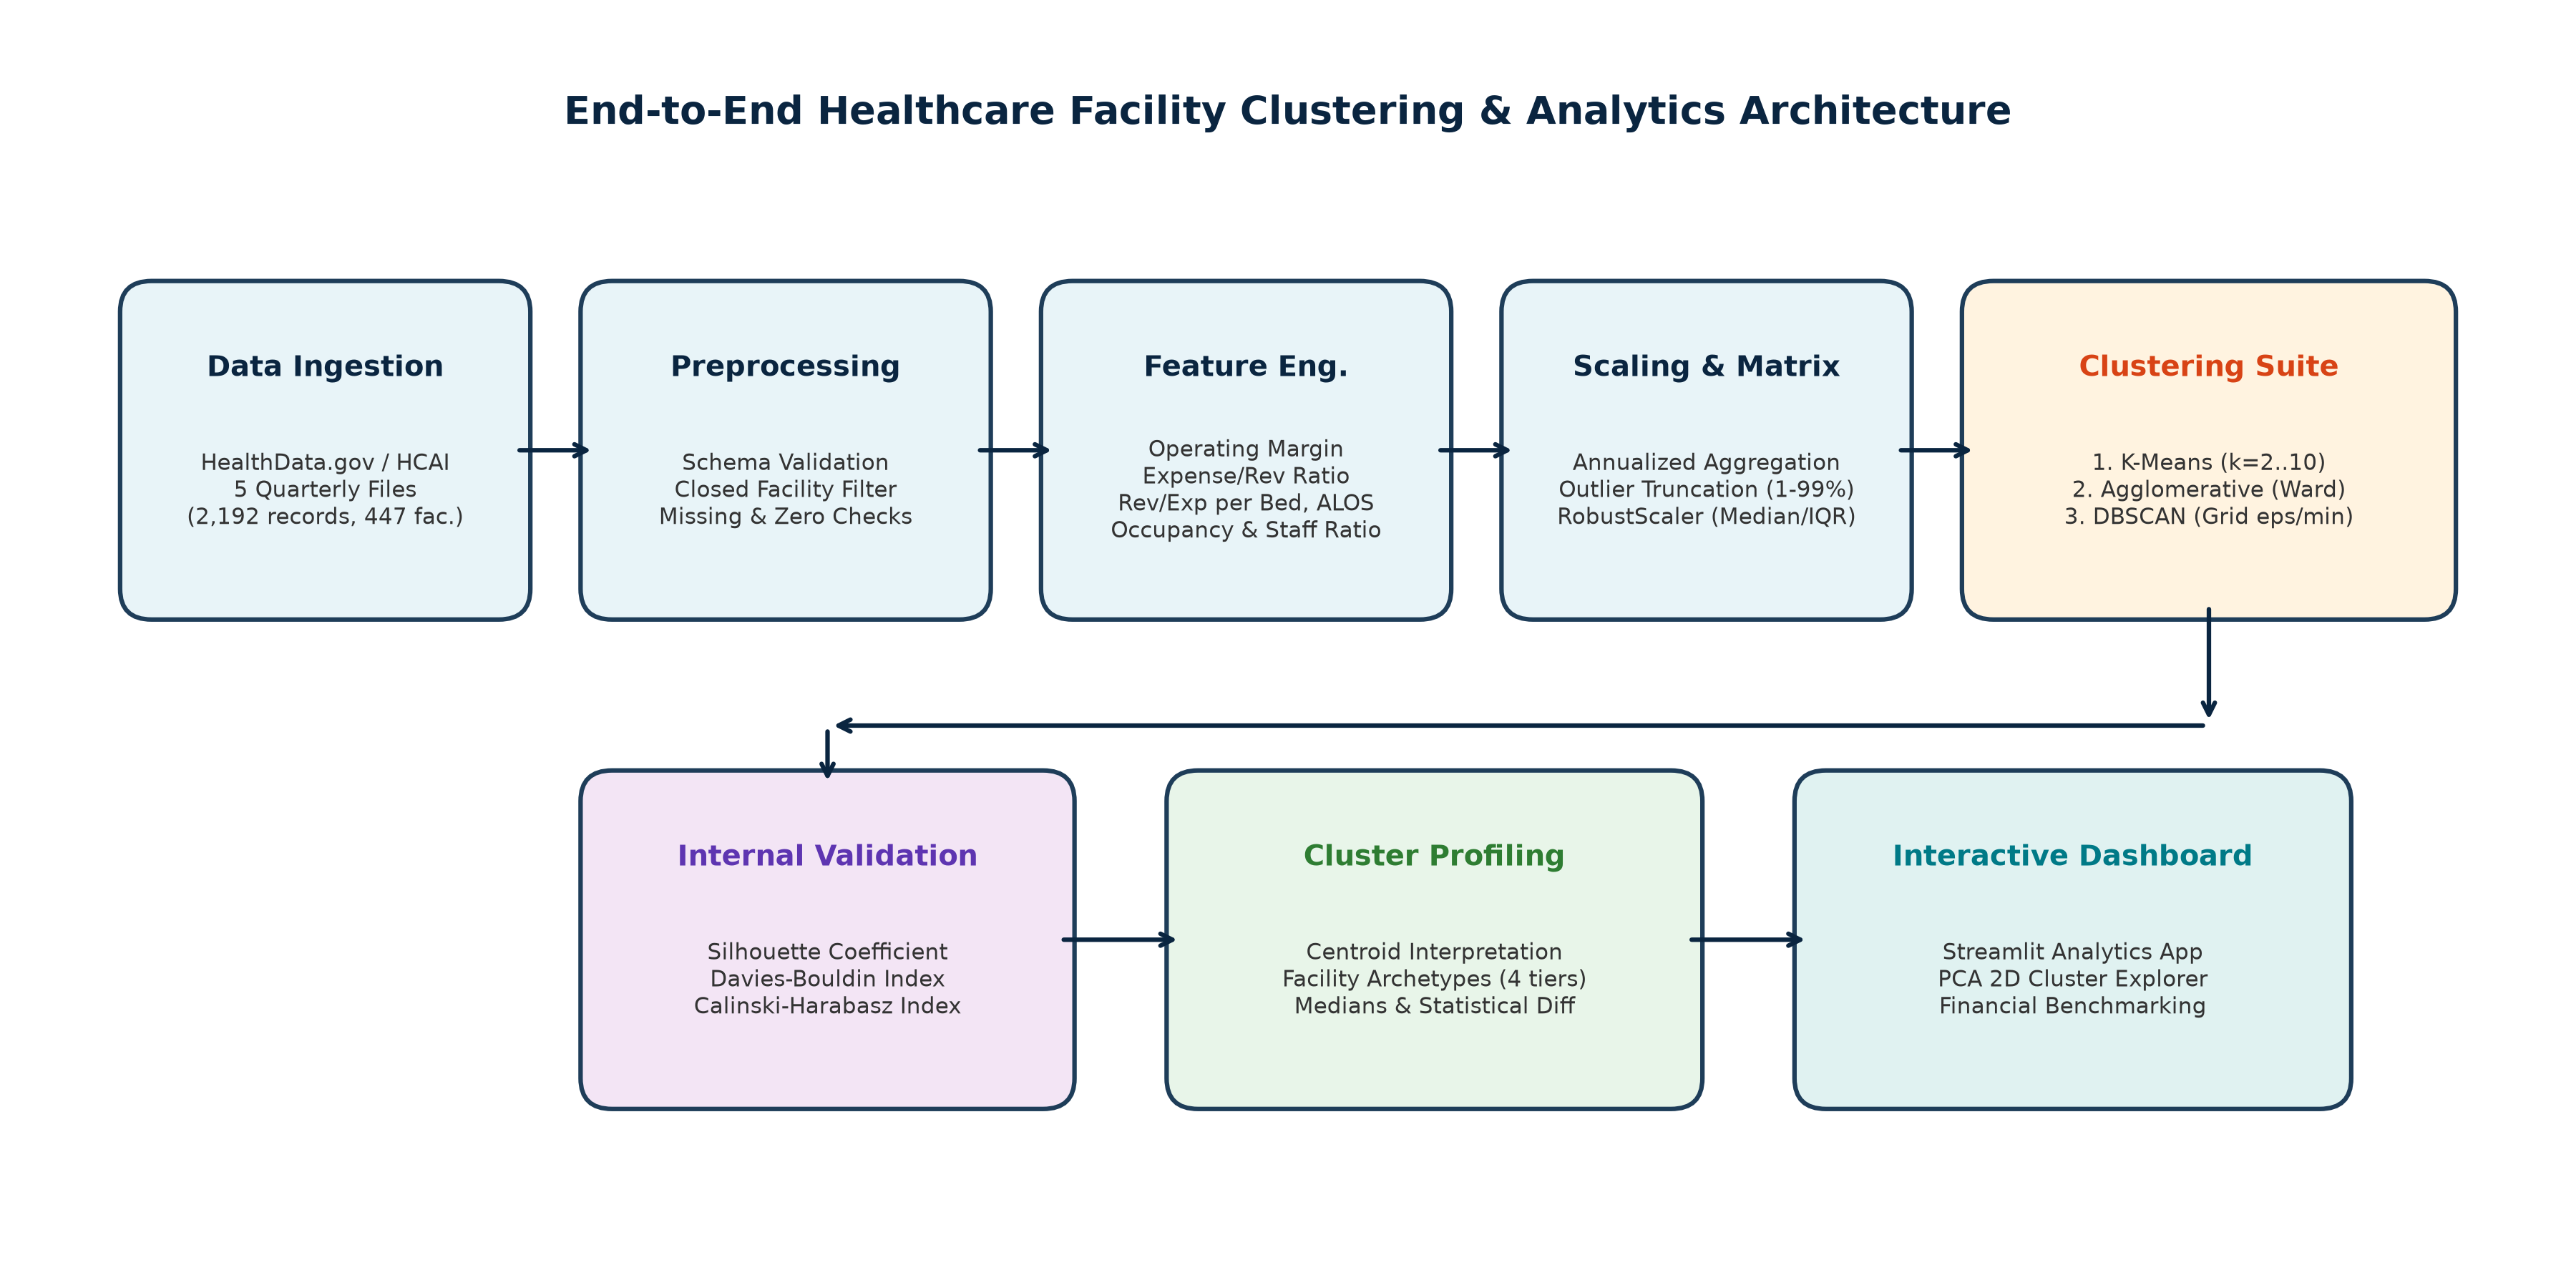
\includegraphics[width=0.95\columnwidth]{figures/architecture_diagram.png}
\caption{End-to-end healthcare facility clustering and analytics architecture.}
\label{fig:arch}
\end{figure}

\subsection{Feature Formulation and Scaling}
We engineered eight indicators: Operating Margin ($OP\_MARGIN$), Expense-to-Revenue Ratio ($EXP\_REV\_RATIO$), Revenue per Bed ($REV\_PER\_BED$), Expense per Bed ($EXP\_PER\_BED$), Bed Occupancy Rate ($OCCUPANCY\_RATE$), Staffed Bed Ratio ($STF\_AVL\_RATIO$), Average Length of Stay ($ALOS$), and Outpatient Ratio ($OUTPATIENT\_RATIO$). Features were winsorized at 1st/99th percentiles and scaled via RobustScaler:
\begin{equation}
x_{\text{scaled}} = \frac{x - Q_2(x)}{Q_3(x) - Q_1(x)}
\end{equation}

\subsection{Clustering Algorithms}
1) \textit{K-Means Objective:} Minimizes total within-cluster sum of squares:
\begin{equation}
J = \sum_{i=1}^n || x_i - \mu_{c_i} ||^2
\end{equation}
2) \textit{Agglomerative Ward Linkage:} Merges clusters $A$ and $B$ minimizing variance growth:
\begin{equation}
\Delta ESS(A, B) = \frac{n_A n_B}{n_A + n_B} || \mu_A - \mu_B ||^2
\end{equation}
3) \textit{DBSCAN:} Identifies core points with $|N_\epsilon(p)| \ge \text{MinPts}$ and assigns density-unreachable points to noise (-1).

\subsection{Internal Validation Metrics}
Silhouette score $s(i) = \frac{b(i) - a(i)}{\max(a(i), b(i))}$, Davies--Bouldin index $DB = \frac{1}{k} \sum_{i=1}^k \max_{j \neq i} \left(\frac{s_i + s_j}{d(\mu_i, \mu_j)}\right)$, and Calinski--Harabasz index $CH = \frac{\text{Tr}(B_k)}{\text{Tr}(W_k)} \frac{n-k}{k-1}$.

\section{Experimental Results and Discussion}
Table~\ref{tab:results} summarizes experimental performance across 64 runs.

\begin{table}[htbp]
\caption{Experimental Clustering Benchmark Comparison (N=428)}
\begin{center}
\begin{tabular}{lcccc}
\toprule
\textbf{Algorithm \& Setting} & \textbf{k} & \textbf{Silhouette} & \textbf{DB Index} & \textbf{CH Index} \\
\midrule
K-Means ($k=2$) & 2 & 0.8818 & 0.3102 & 950.29 \\
K-Means ($k=3$) & 3 & 0.7601 & 0.4741 & 709.62 \\
\textbf{K-Means (Selected, $k=4$)} & \textbf{4} & \textbf{0.6113} & \textbf{0.5768} & \textbf{655.84} \\
K-Means ($k=5$) & 5 & 0.5033 & 0.8612 & 623.68 \\
Agglomerative (Ward, $k=4$) & 4 & 0.6708 & 0.4634 & 638.75 \\
Agglomerative (Avg, $k=4$) & 4 & 0.7005 & 0.4660 & 524.36 \\
DBSCAN ($\epsilon=1.8, \text{MinPts}=3$) & 2 & 0.9352 & 0.0615 & 1522.79 \\
\bottomrule
\end{tabular}
\label{tab:results}
\end{center}
\end{table}

\begin{figure}[htbp]
\centering
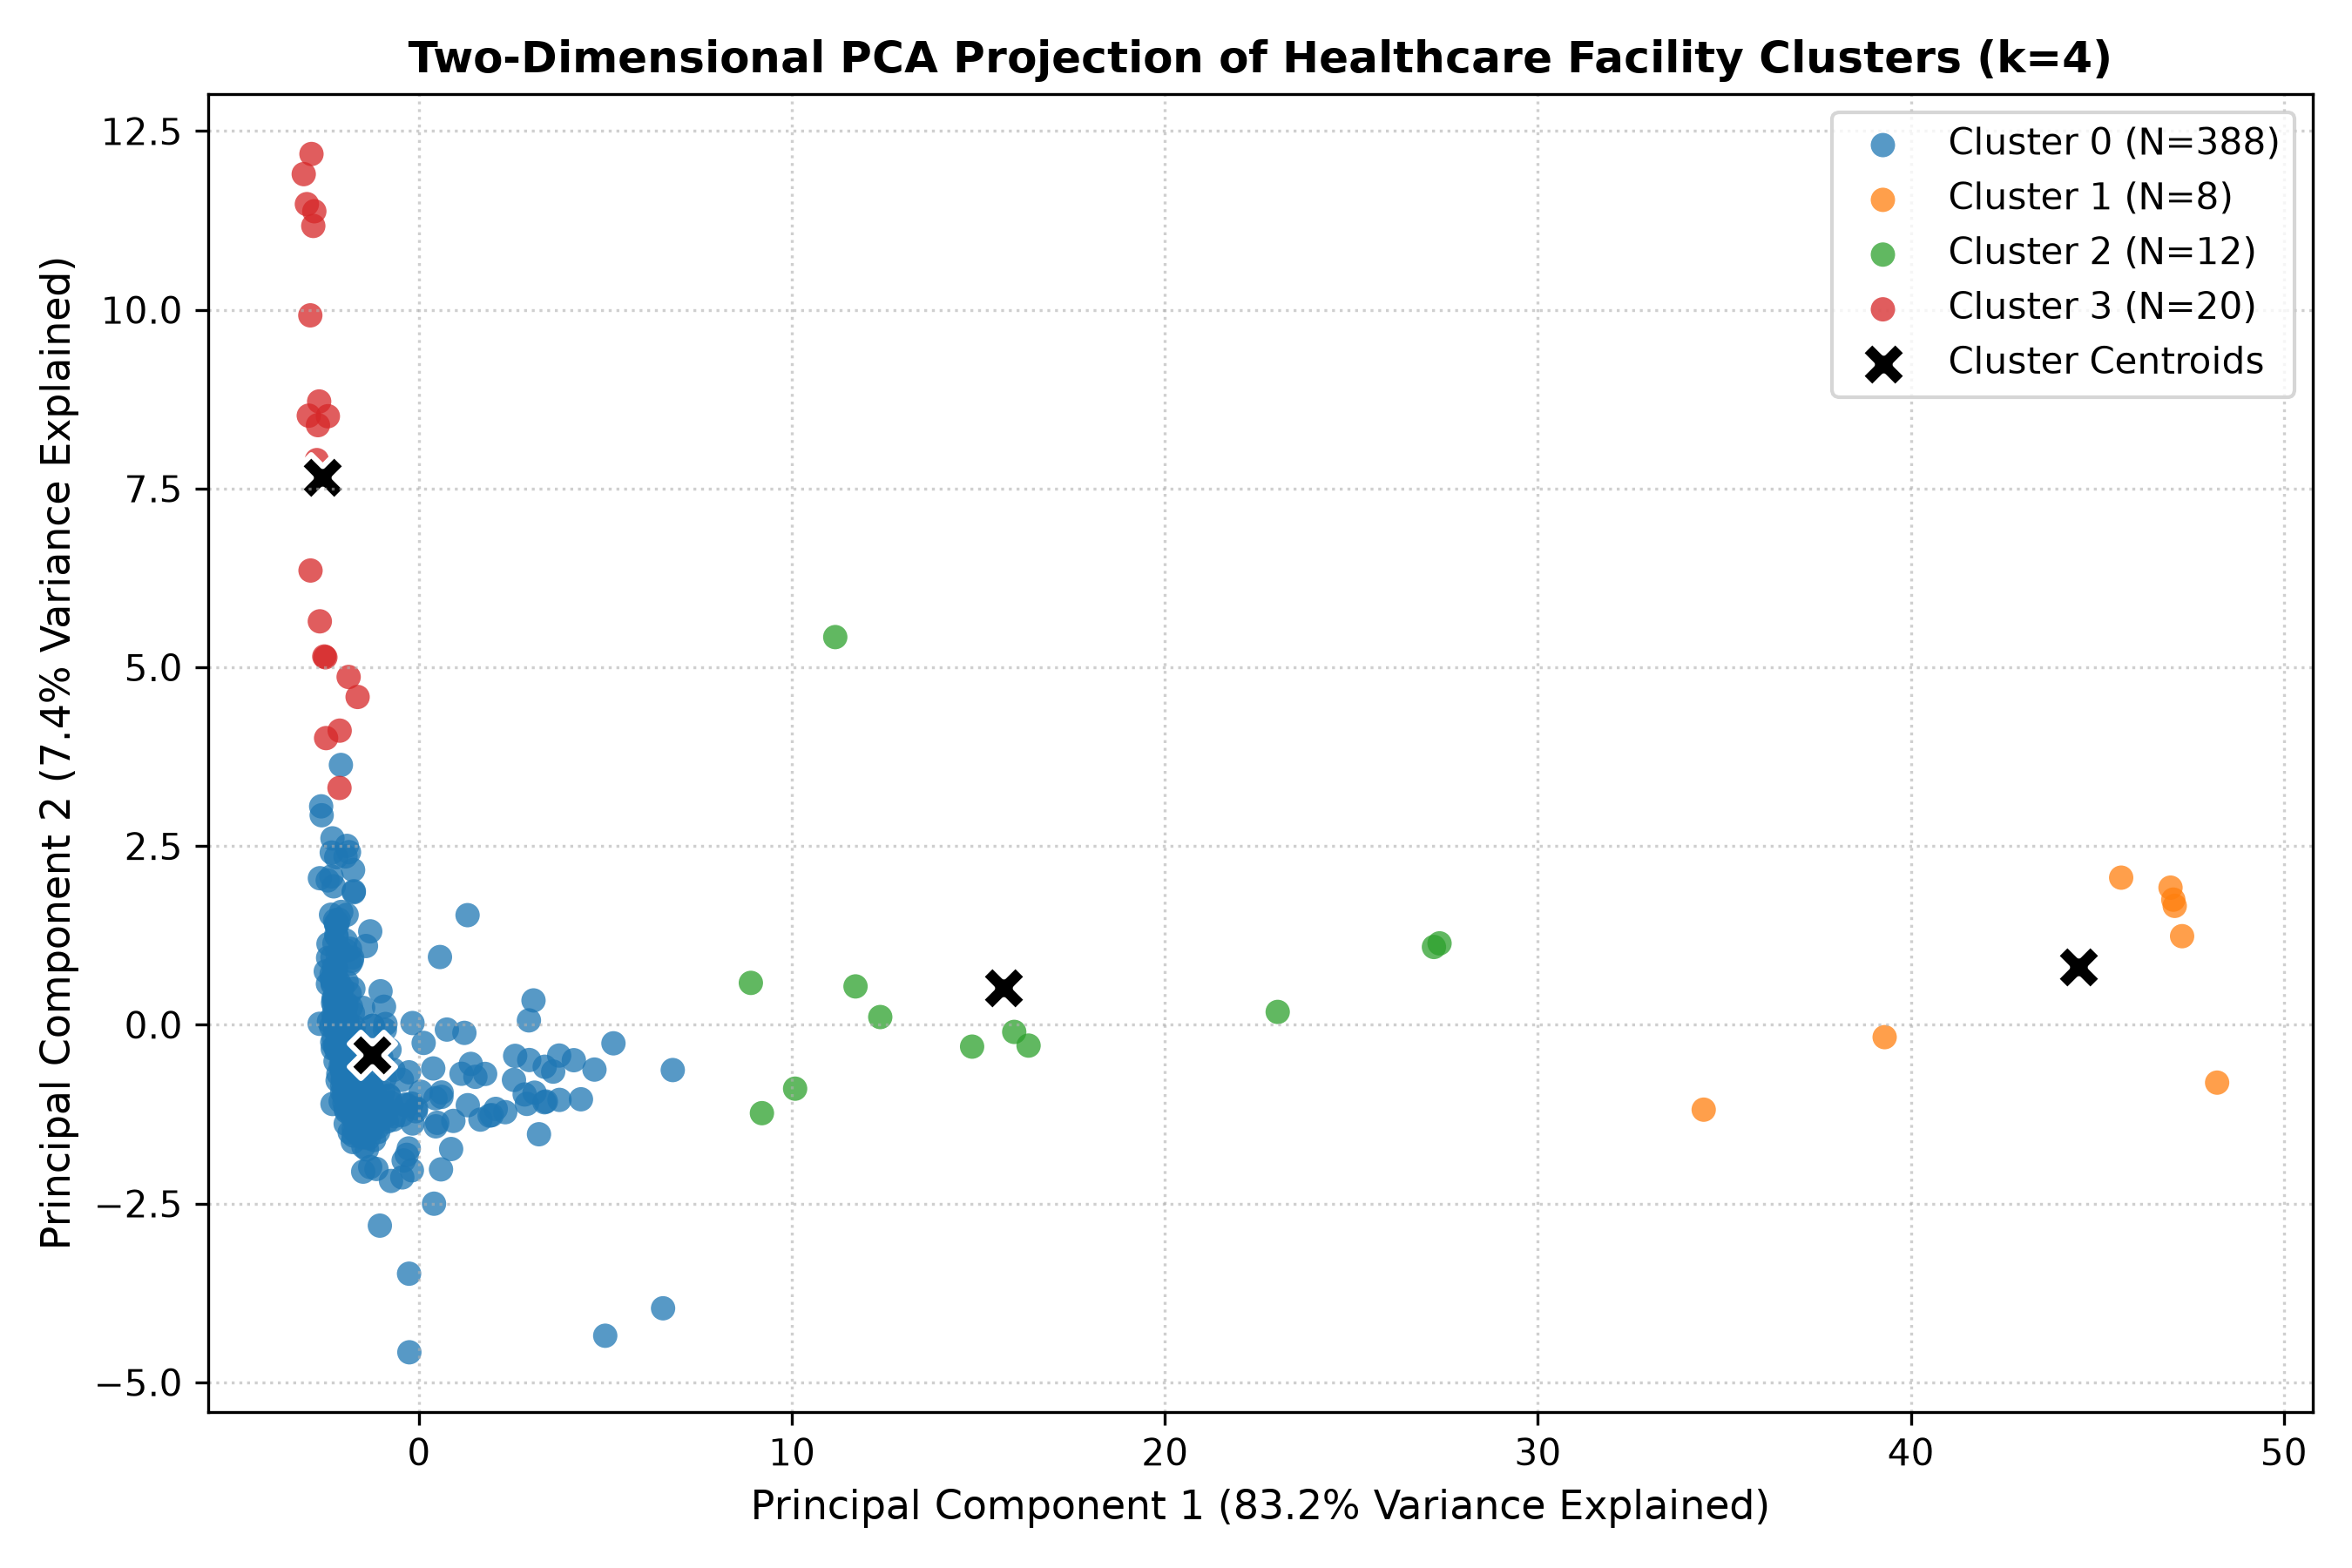
\includegraphics[width=0.9\columnwidth]{figures/pca_clusters.png}
\caption{Two-dimensional PCA projection of facility clusters ($k=4$).}
\label{fig:pca}
\end{figure}

\begin{table}[htbp]
\caption{Empirical Cluster Profiles (Median Values)}
\begin{center}
\begin{tabular}{lcccc}
\toprule
\textbf{Profile} & \textbf{N (\%)} & \textbf{Margin} & \textbf{Rev/Bed} & \textbf{ALOS} \\
\midrule
Cluster 0: General Acute & 388 (90.7\%) & +0.93\% & \$1,307,873 & 5.7 d \\
Cluster 1: State / Long-Term & 8 (1.9\%) & -48.20\% & \$217,376 & 403.2 d \\
Cluster 2: Subacute Rehab & 12 (2.8\%) & -9.46\% & \$361,768 & 122.2 d \\
Cluster 3: Specialized Surgical & 20 (4.7\%) & +3.12\% & \$3,575,897 & 3.6 d \\
\bottomrule
\end{tabular}
\label{tab:profiles}
\end{center}
\end{table}

\section{Conclusion and Ethical Considerations}
This study established an empirical facility segmentation across California healthcare institutions. K-Means at $k=4$ reveals that over 90\% of community acute hospitals operate on slim margins ($+0.93\%$), while specialized surgical centers capitalize on rapid throughput and high capital turnover. These findings reflect descriptive statistical associations and do not imply clinical quality or individual patient outcomes.

\bibliographystyle{IEEEtran}
\bibliography{references}

\end{document}
